\documentclass[../main.tex]{subfiles}
\begin{document}

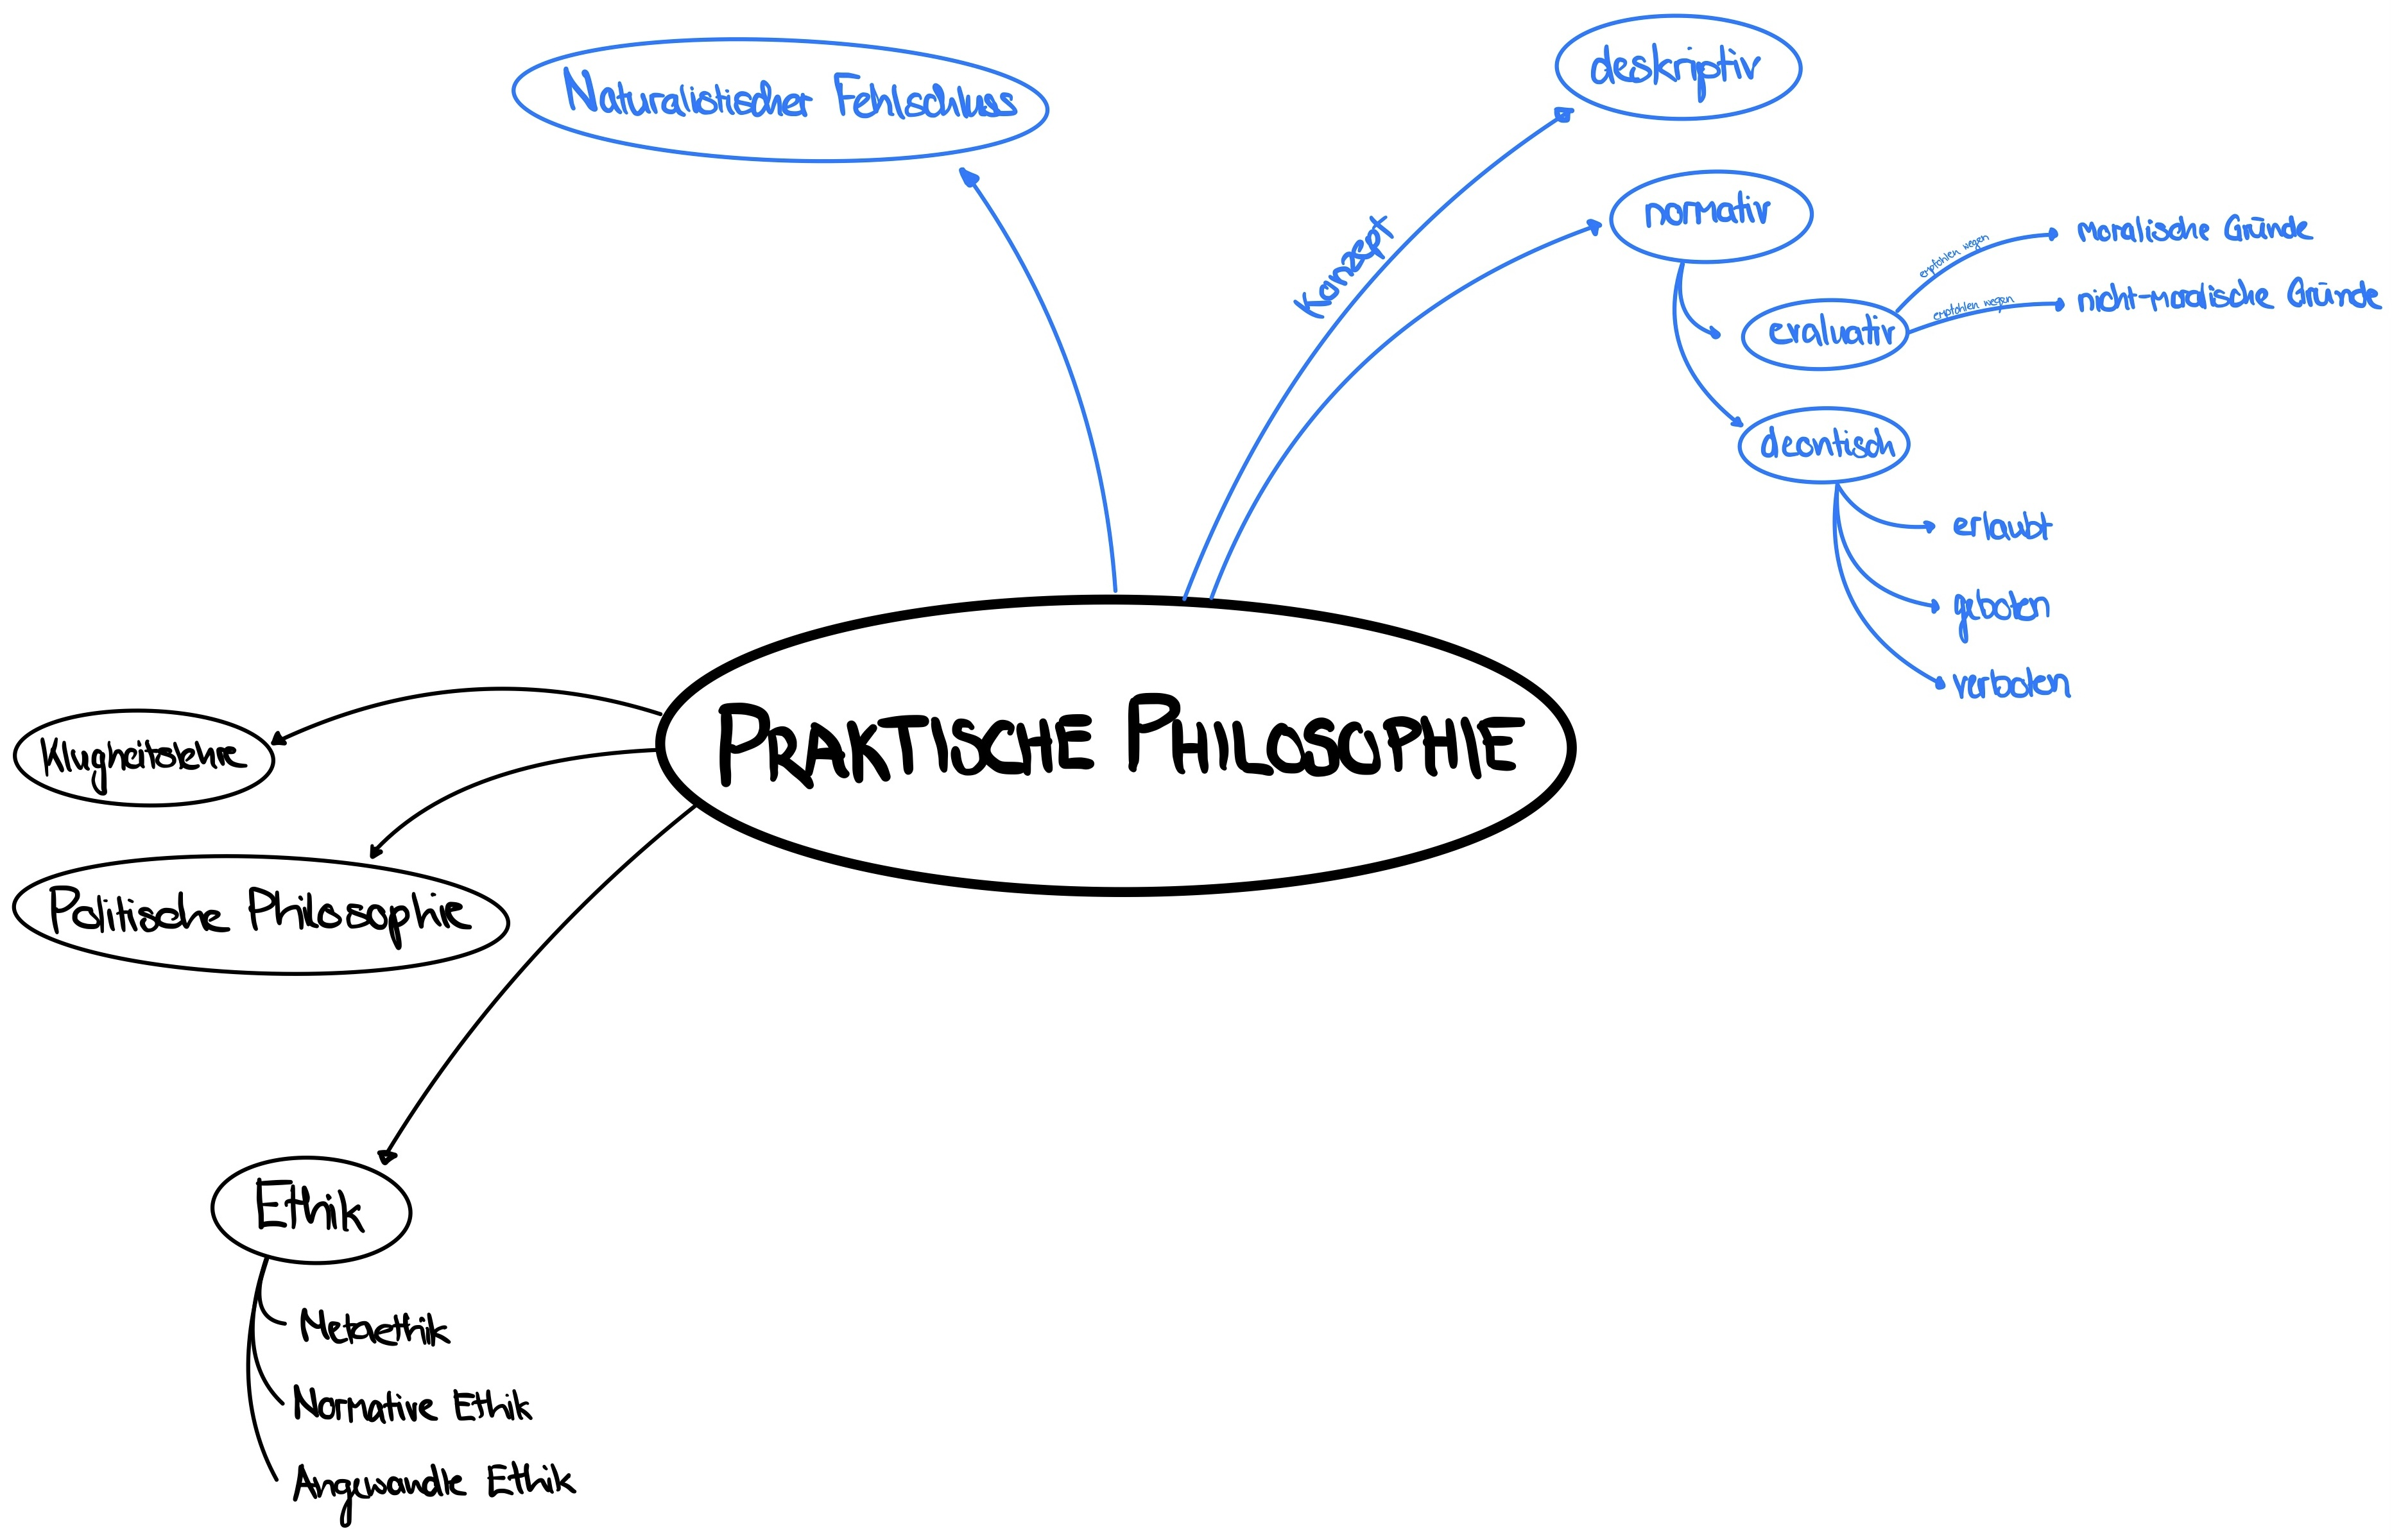
\includegraphics[width=\textwidth]{images/Uebersicht_Einf_Praktische_Philosophie.jpg}

\section{Gebiete der Philosophie}
\paragraph{Klugheitslehre}
\textit{Wie führt man ein glückliches Leben?}

\paragraph{Politische Philosophie}
Bestimmung der Prinzipien des Zusammenlebens (Staat, Recht, Besteuerung, etc.)

\paragraph{Ethik}
\begin{itemize}
  \item Metaethik \\
Theorien ohne Moral; Es wird versucht objektiv die Natur von Moral zu ergründen. \textit{Was ist Wahrheit? \\Lässt sich recht/unrecht definieren? \\Gibt es Moral und wenn ja, ist sie konstruiert oder eine von uns unabhängige Instanz?}
  \item Normative Ethik \\
Theorien der Moral, Prinzipien des moralischen Handelns. \textit{Ist das richtig?}
  \item Angewandte Ethik \\ Konkrete Detailfragen werden behandelt. \textit{Was ist in dieser Situation richtig/falsch?}
\end{itemize}

\section{Sprachliche Grunddefinitionen}

\subsubsection{normativ} \label{normative}
\begin{warningbox}
Normative Aussagen (was sein soll) sind \textbf{Bewertungen}, können also weder wahr noch falsch sein. Man kann sich ihnen gegenüber (bezogen auf den wertenden Inhalt) richtig oder falsch verhalten.
\end{warningbox}
Normative Aussagen (NA) beschreiben, \textit{wie die Welt sein soll}. Es wird unterschieden zwischen \textbf{evaluativen} Aussagen, die durch eine Wertung, basierend auf moralischen oder nicht-moralischen Gründen gemäss \ref{moralAndNonMoralReasons}, eine Empfehlung ausdrücken und \textbf{deontischen} Aussagen, die besagen, ob etwas erlaubt (E), geboten (G) oder verboten (V) ist.


\subsubsection{deskriptiv} \label{descriptive}
\begin{warningbox}
Deskriptive Aussagen (was ist) sind \textbf{Beschreibungen}, können also wahr noch falsch sein. Man kann sie (ihren informativen Gehalt) nur ablehnen oder annehmen. 
\end{warningbox}
Deskriptive Aussagen beschreiben, \textit{wie die Welt ist}.


\subsubsection{Moralische und nicht-moralische Gründe} \label{moralAndNonMoralReasons}
Evaluative Aussagen gemäss \ref{normative} gliedern sich aufgrund ihrer Begründung in moralische und nicht-moralische Empfehlungen. Werden moralische Gründe aufgeführt, steht zur Diskussion, ob sich aus diesen eine moralische Empfehlung oder eine moralische Pflicht ableiten lässt. 
\\\textit{Pflicht} bedeutet, dass die Unterlassung verboten resp. die Handlung geboten ist, moralische Vorwürfe bei Unterlassung erhoben werden können/dürfen und die Handlung gefordert werden kann. 
\\\textit{Nicht meine Pflicht} bedeutet, dass kein moralischer Vorwurf erhoben werden darf/kann, sollte man nicht handeln. Handeln ohne Pflicht, also Handeln über die Pflichterfüllung hinaus, nennt man \textbf{supererogatorisch}.

\subsubsection{Harmless wrongdoing}
Als \textit{harmless wrongdoing} wird eine Handlung bezeichnet, die unrecht ist, der betroffenen Person aber nicht schadet.

\section{Naturalistischer Fehlschluss}
\begin{warningbox}
Aus deskriptiven Aussagen lassen sich keine normative Aussagen ableiten.
\end{warningbox}
Der naturalistische Fehlschluss beschreibt die Tätigkeit, dass ohne Prämisse (einleitende Annahme, was \textit{gut} ist) aus deskriptiven Aussagen (gem. \ref{descriptive}) eine normative Aussage Abgeleitet wird. 


\end{document}